In this section, we present the final results for each individual verilog filed we have submitted:



\subsection{Multi stage path for delay measurements}
The multi stage path was submitted with no errors, and the final layout is shown in figure\ \ref{fig:delay_Layout}. The final layout is composed of 4 stages, each stage has 4 inverters and 4 transmission gates.
\begin{figure}[H]
    \centering
    \begin{subfigure}[b]{0.45\textwidth}
        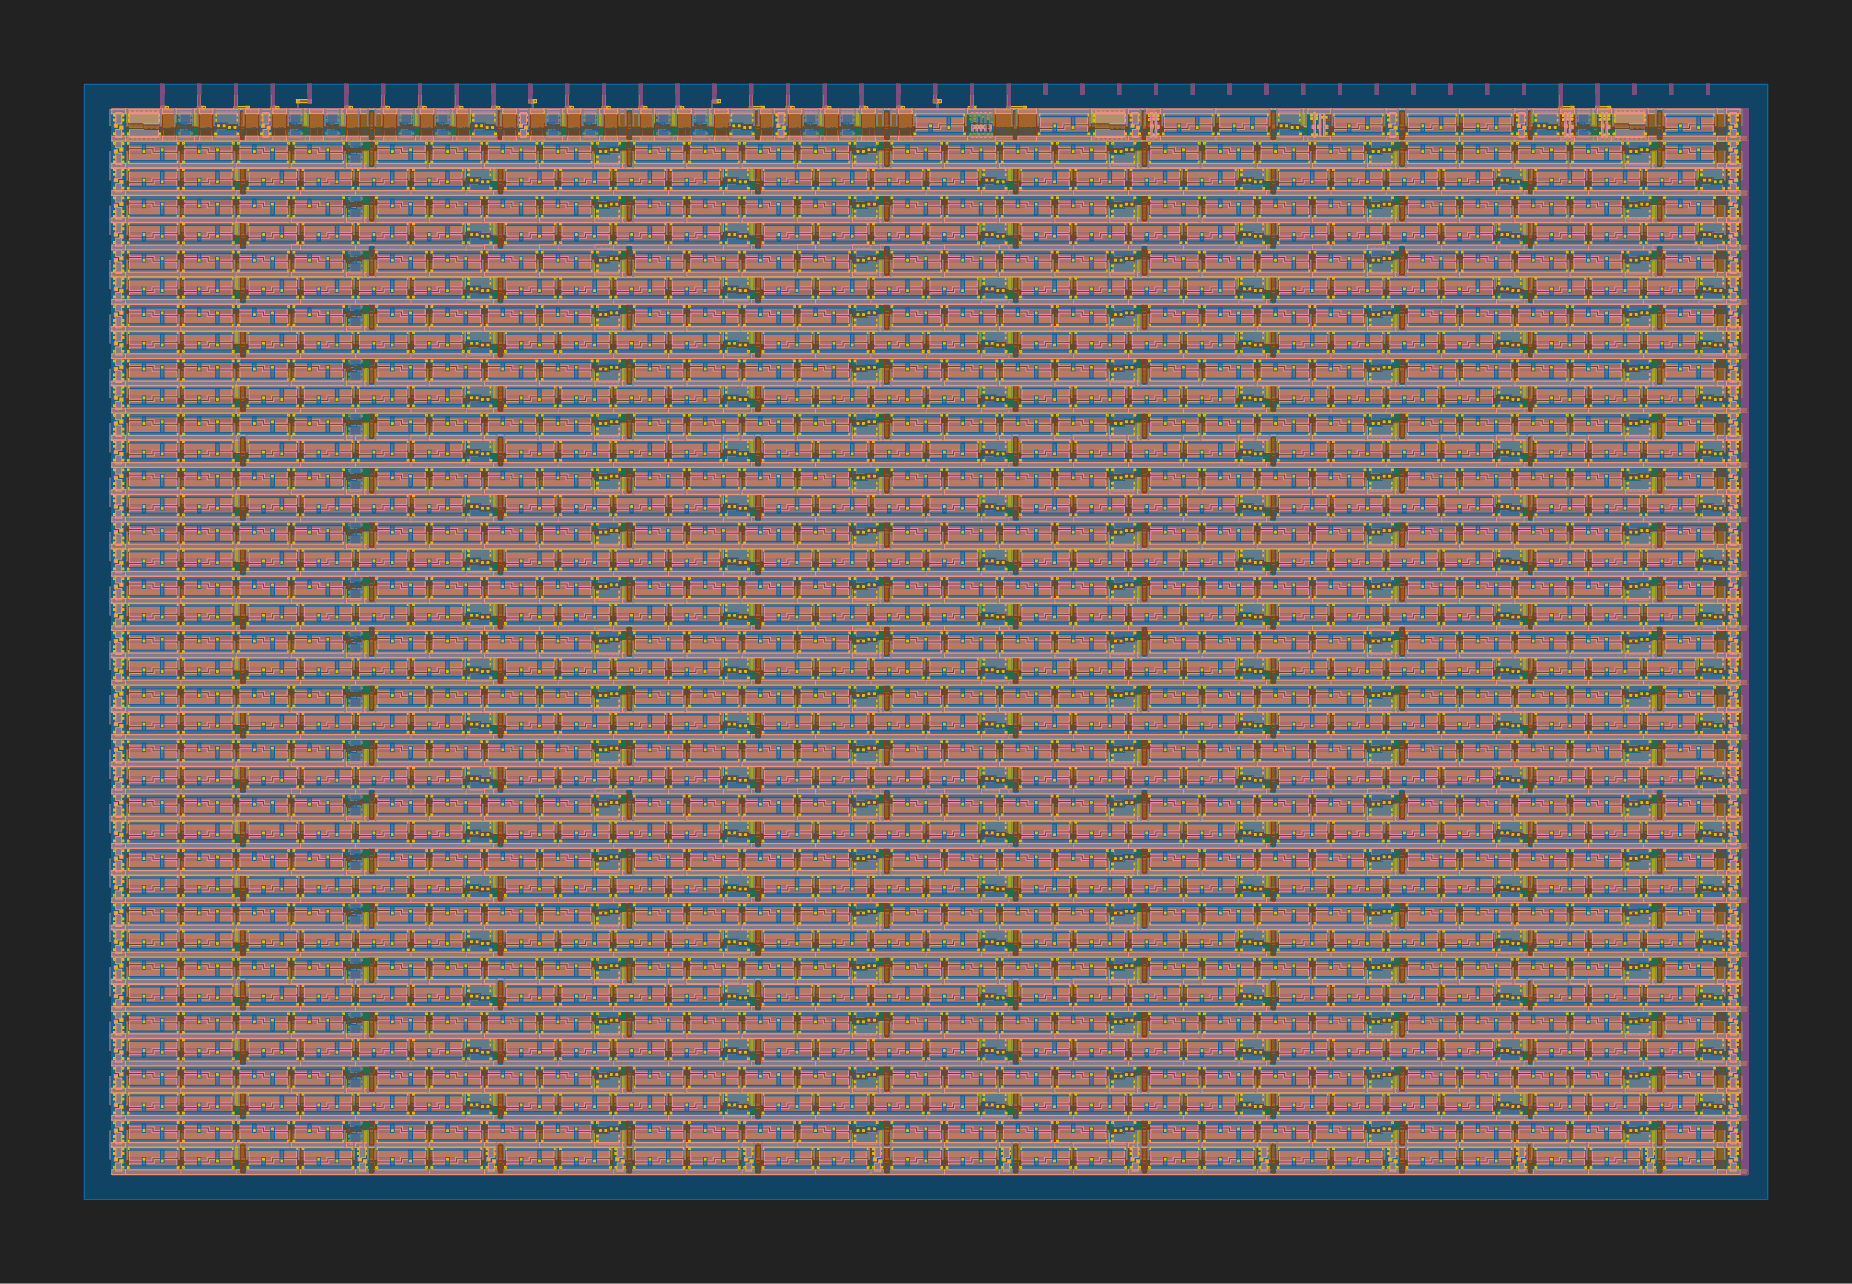
\includegraphics[width=\linewidth]{Pictures/Result_Delay_2D_View.png}
        \caption{View 2D}\label{fig:delay_2D}
    \end{subfigure}
    \begin{subfigure}[b]{0.45\textwidth}
        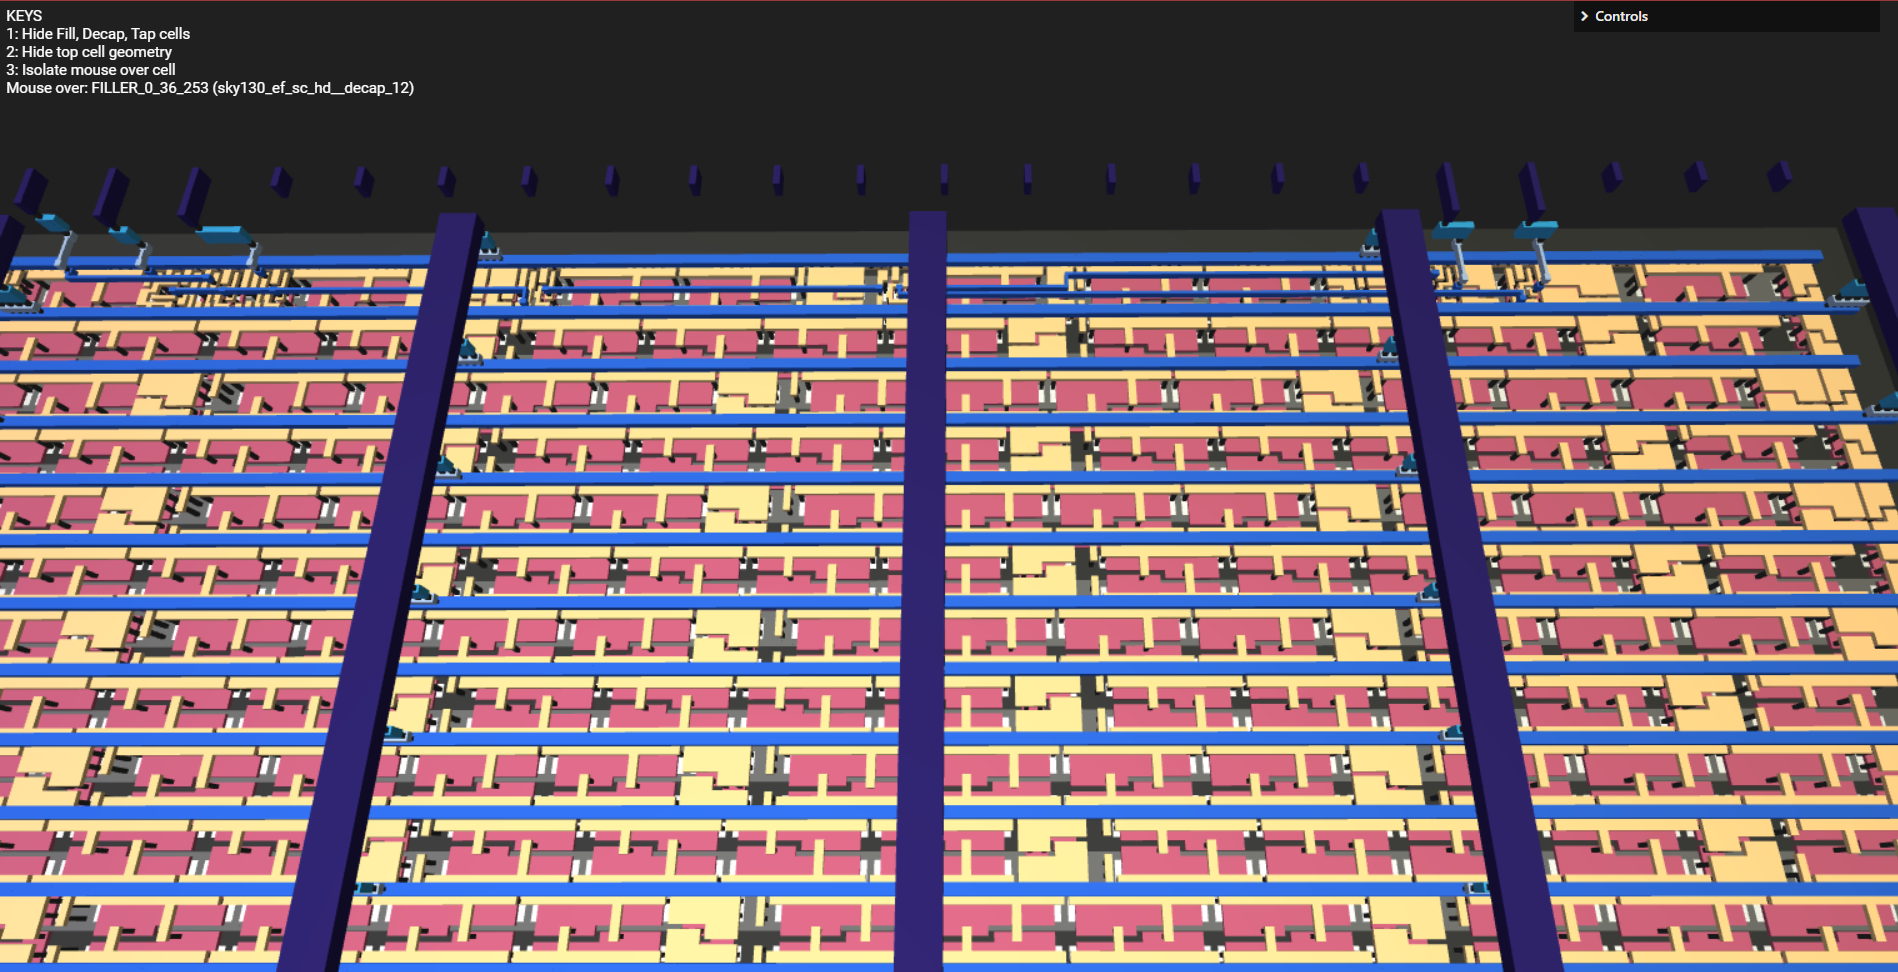
\includegraphics[width=\linewidth]{Pictures/Result_Delay_3D_View.png}
        \caption{View 3D}\label{fig:delay_3D}
    \end{subfigure}
    \caption{Multi stage path for delay measurements layout}\label{fig:delay_Layout}
\end{figure}

\subsection{ASCII Text Printer Circuit}
The circuit ASCII text printer was submitted with no errors, and the final layout is shown in figure\ \ref{fig:ASCII_Layout}.
\begin{figure}[H]
    \centering
    \begin{subfigure}[b]{0.45\textwidth}
        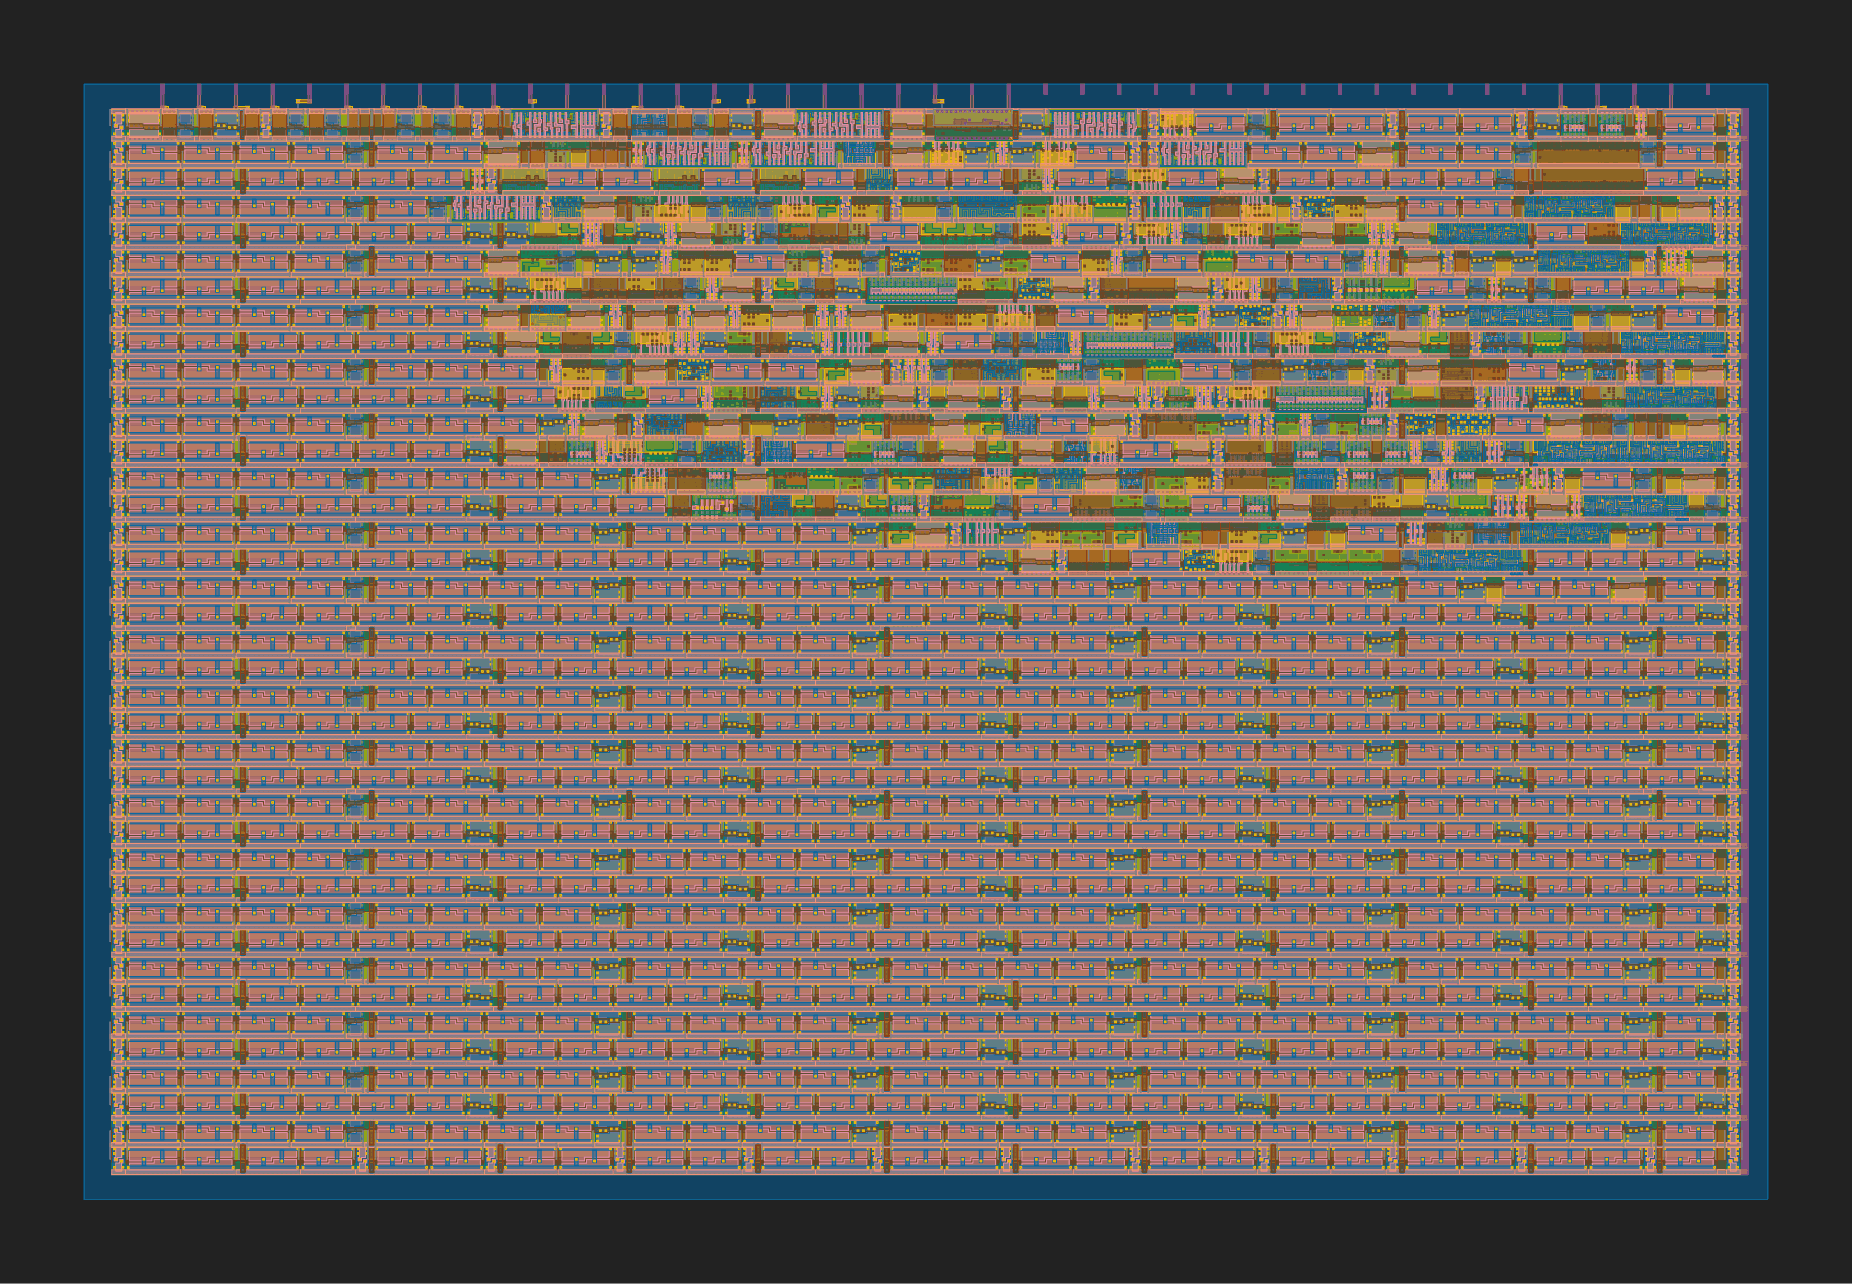
\includegraphics[width=\linewidth]{Pictures/Result_ASCII_2D_View.png}
        \caption{View 2D}\label{fig:ASCII_2D}
    \end{subfigure}
    \begin{subfigure}[b]{0.45\textwidth}
        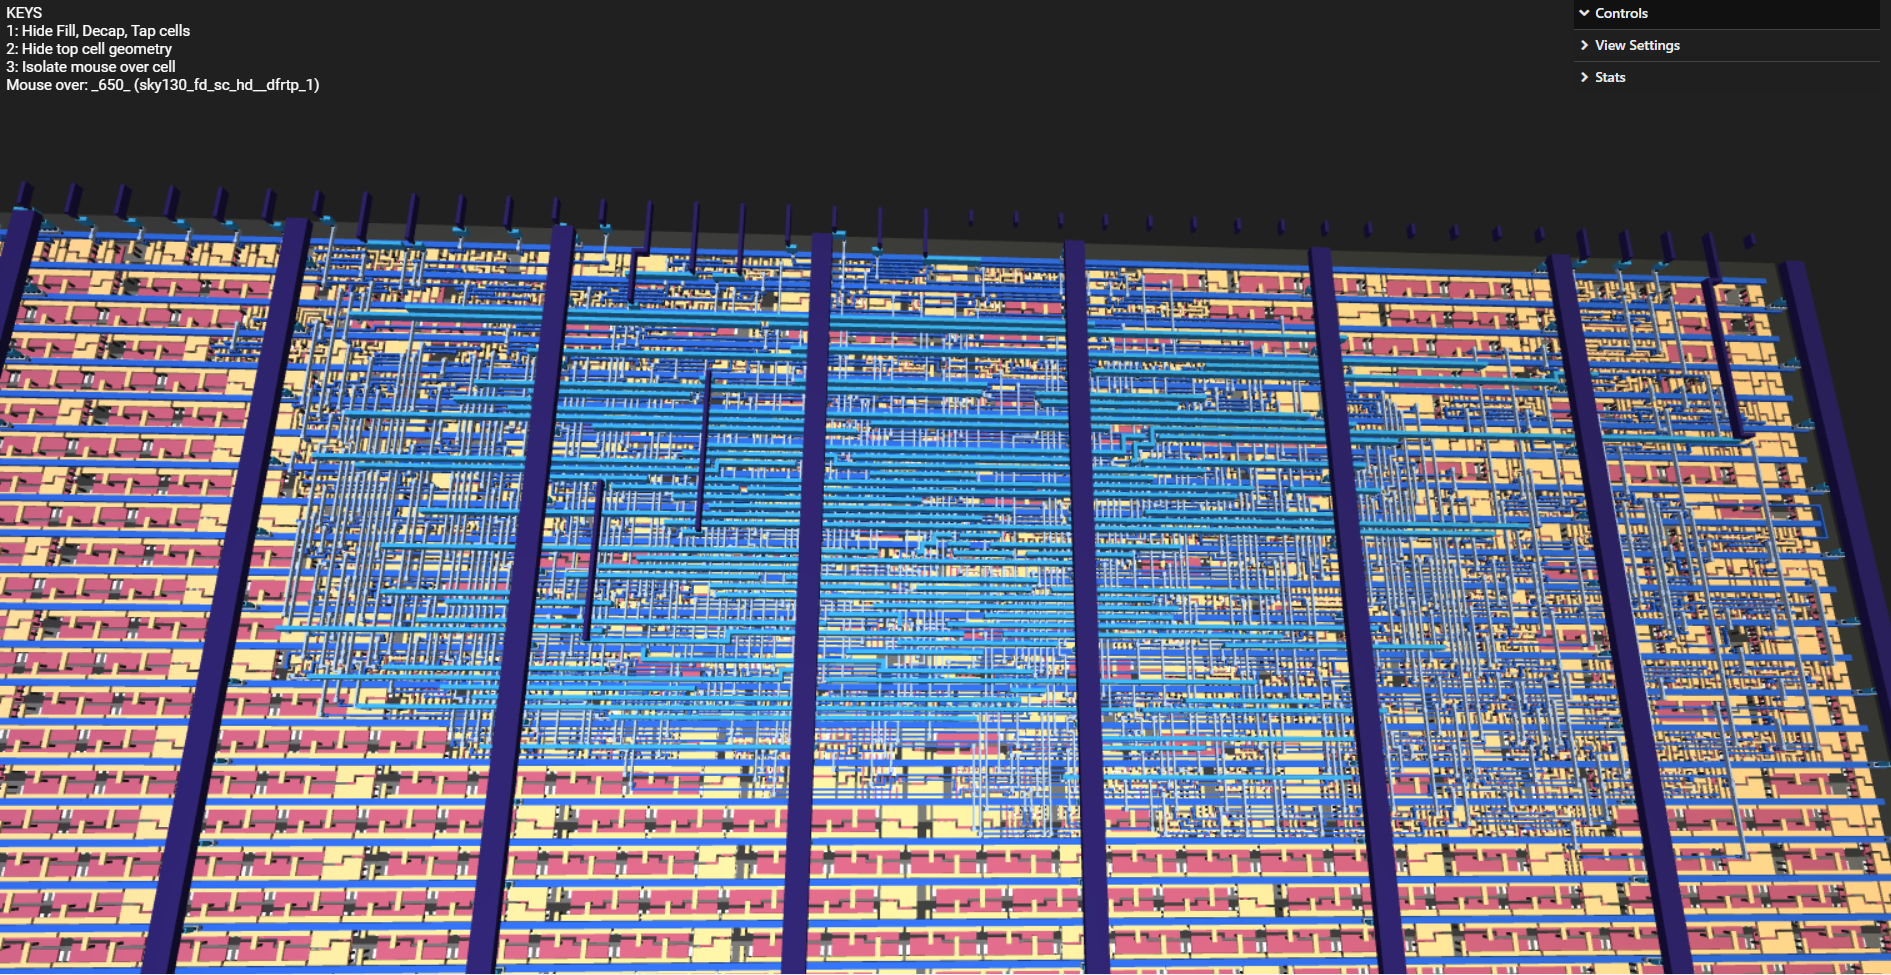
\includegraphics[width=\linewidth]{Pictures/Result_ASCII_3D_View.png}
        \caption{View 3D}\label{fig:ASCII_3D}
    \end{subfigure}
    \caption{ASCII text printer circuit layout}\label{fig:ASCII_Layout}
\end{figure}

\subsection{Implementation of the Pong game}

\begin{figure}[H]
    \centering
    \begin{subfigure}[b]{0.45\textwidth}
        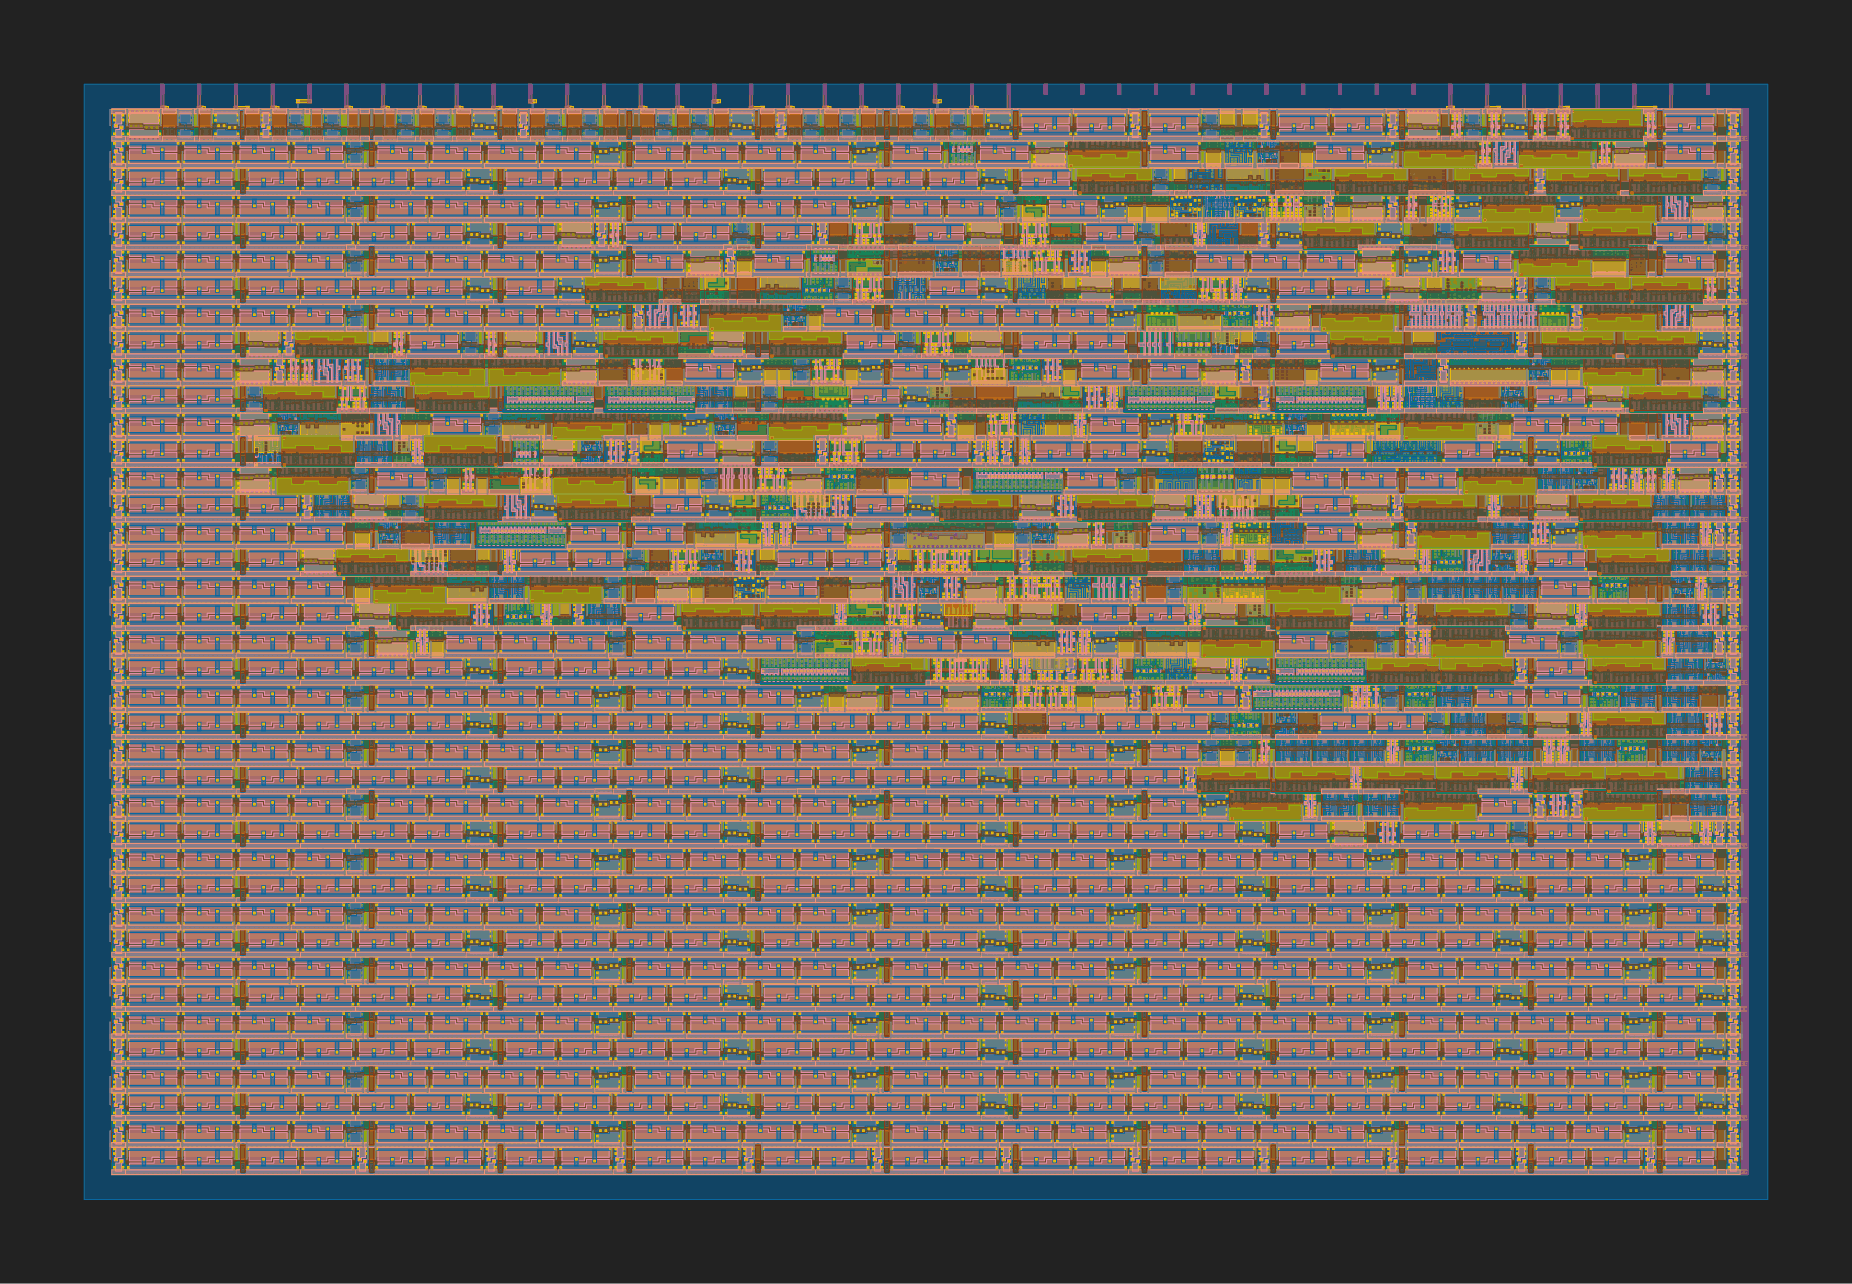
\includegraphics[width=\linewidth]{Pictures/Result_Pong_2D_View.png}
        \caption{View 2D}\label{fig:pong_2D}
    \end{subfigure}
    \begin{subfigure}[b]{0.45\textwidth}
        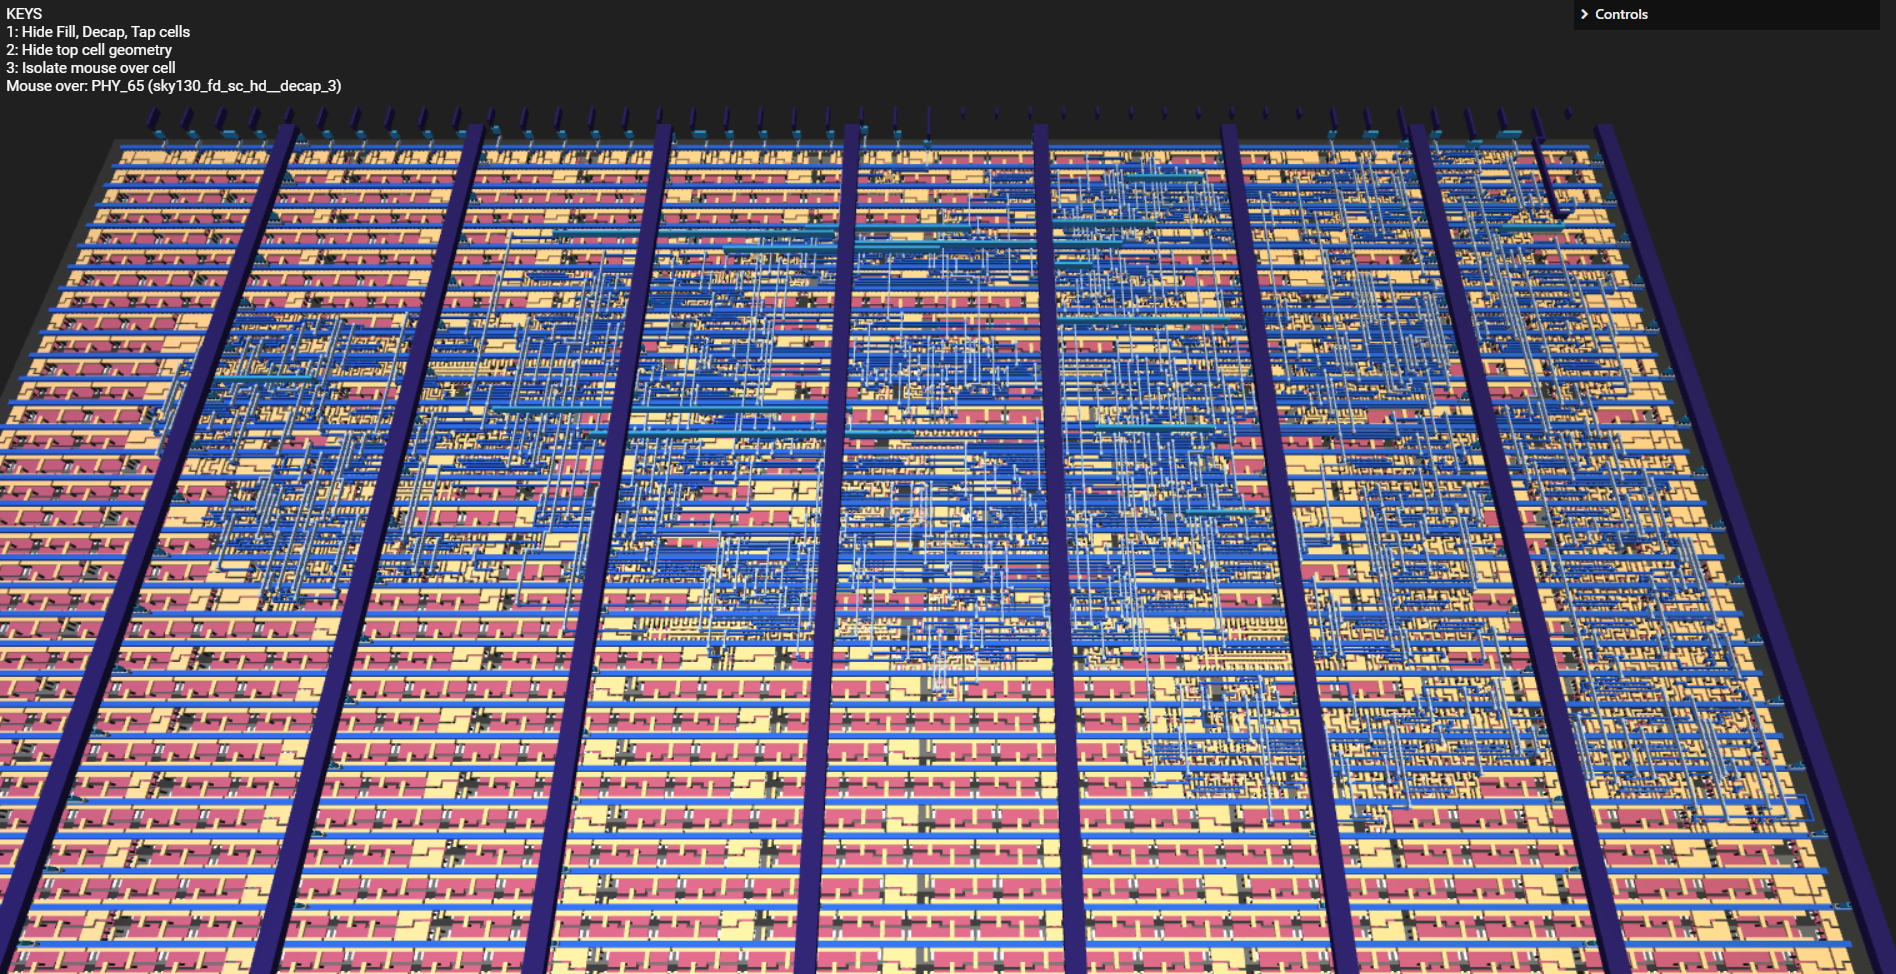
\includegraphics[width=\linewidth]{Pictures/Result_Pong_3D_View.png}
        \caption{View 3D}\label{fig:pong_3D}
    \end{subfigure}
    \caption{The Pong game layout}\label{fig:Pong_Layout}
\end{figure}

\subsection{Pulse Width Modulation Generator}

\begin{figure}[H]
    \centering
    \begin{subfigure}[b]{0.45\textwidth}
        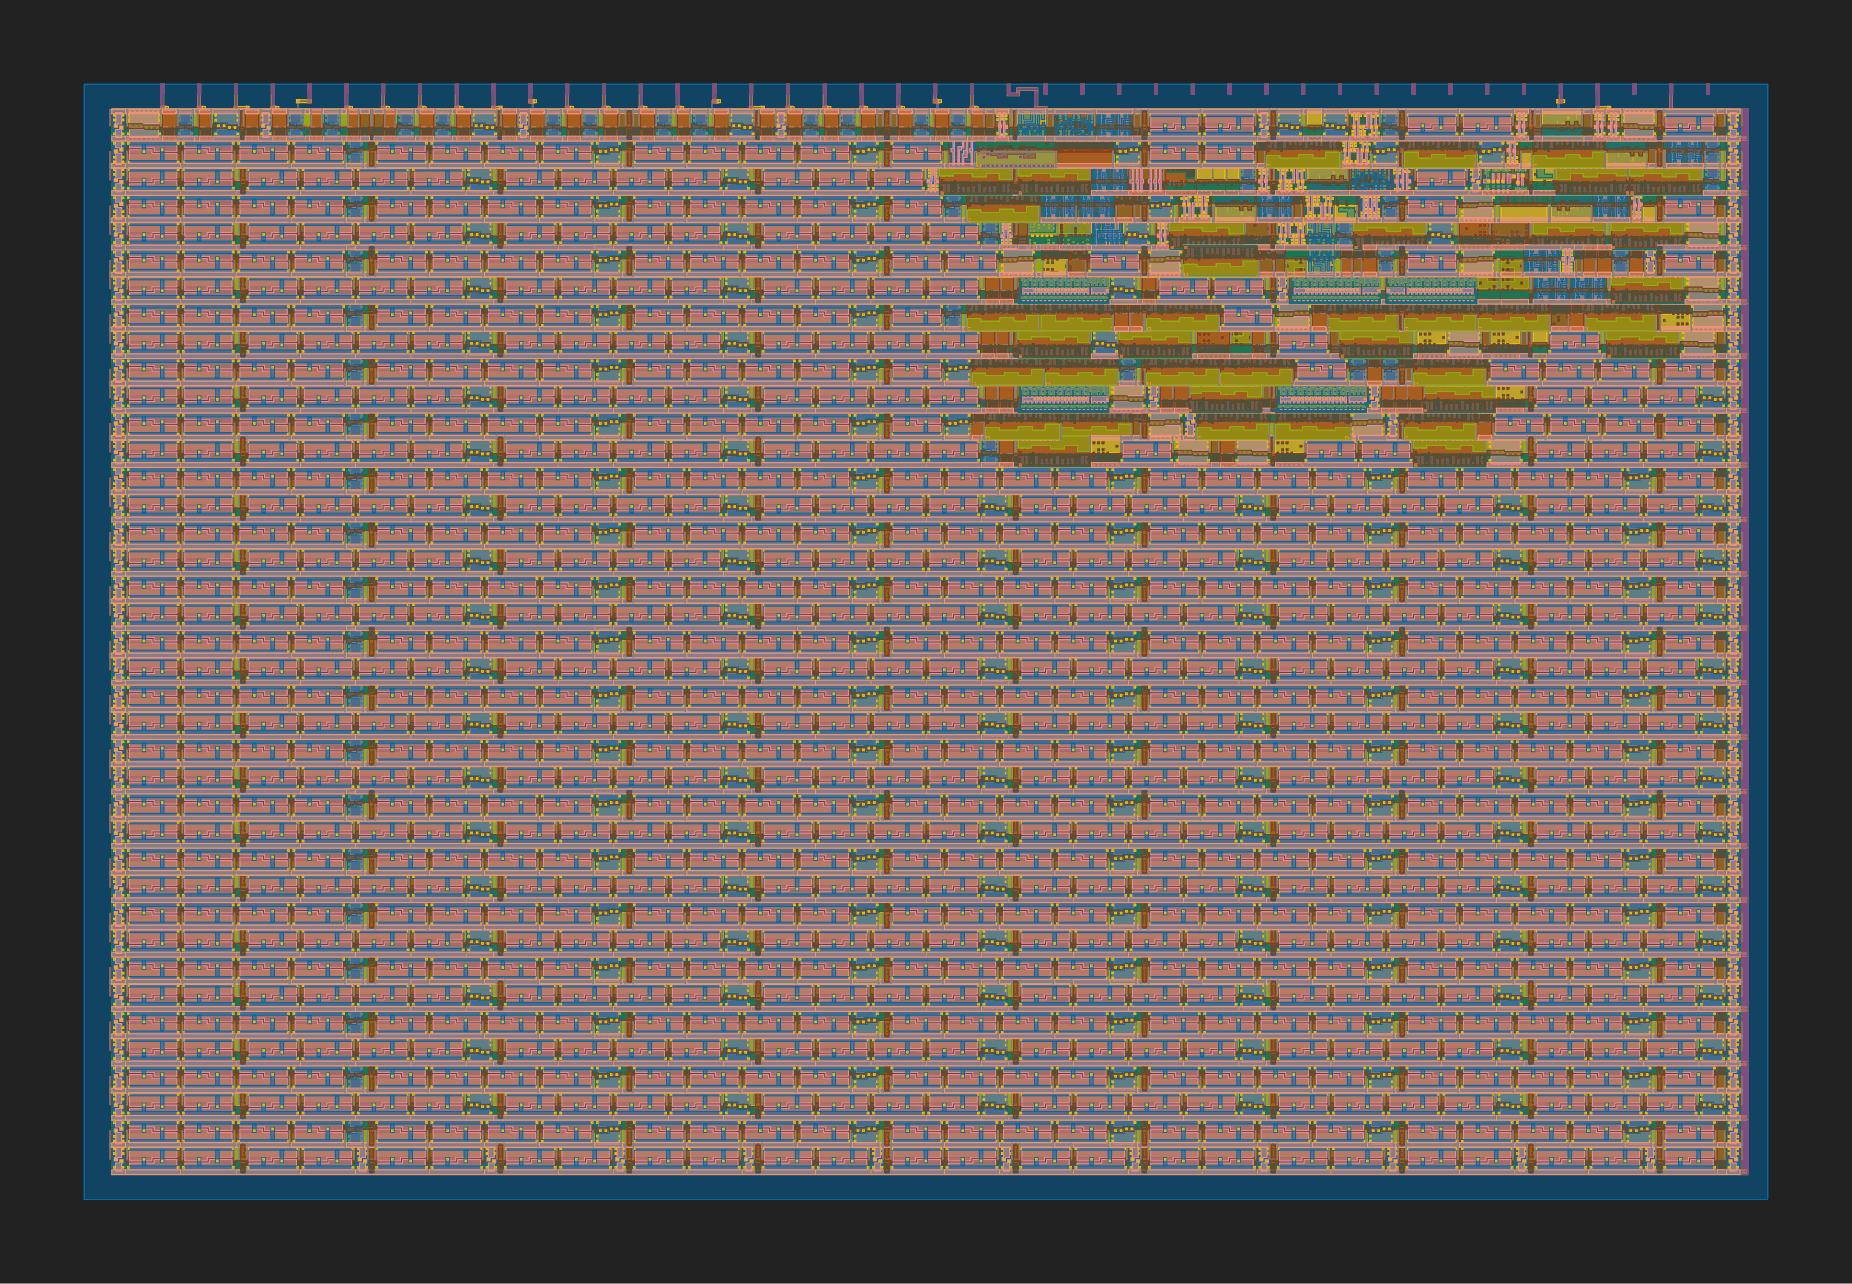
\includegraphics[width=\linewidth]{Pictures/Result_PWM_2D_View.png}
        \caption{View 2D}\label{fig:PWM_2D}
    \end{subfigure}
    \begin{subfigure}[b]{0.45\textwidth}
        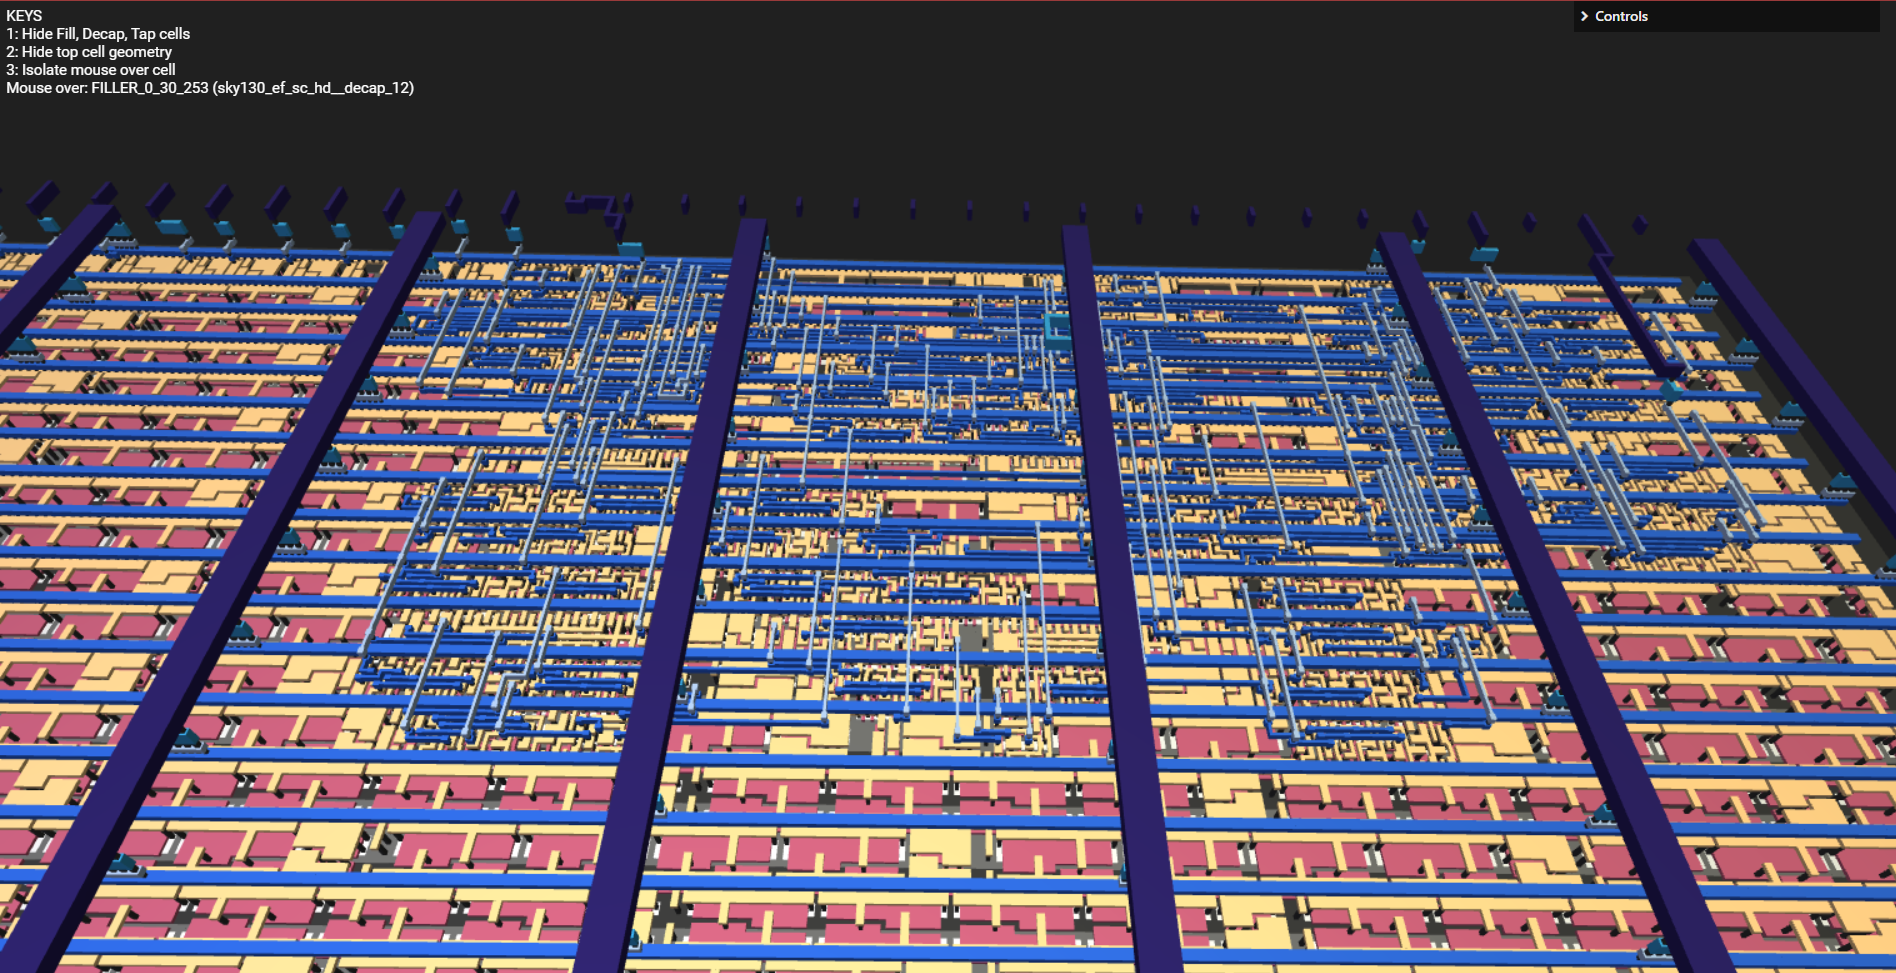
\includegraphics[width=\linewidth]{Pictures/Result_PWM_3D_View.png}
        \caption{View 3D}\label{fig:PWM_3D}
    \end{subfigure}
    \caption{Pulse Width Modulation generator layout}\label{fig:PWM}
\end{figure}

% Please add the following required packages to your document preamble:
% \usepackage{graphicx}
\begin{table}[H]
    \centering
    \resizebox{\columnwidth}{!}{%
    \begin{tabular}{cc}
    \hline
    Circuit                                 & Porcentage utilize(\%) \\ \hline
    Multi stage path for delay measurements & 0.63                  \\
    ASCII Text Printer Circuit              & 17.87                 \\
    Implementation of the Pong game         & 28.82                 \\
    Pulse Width Modulation Generator        & 9.59                  \\ \hline
    \end{tabular}%
    }
    \caption{Porcentaje utilize in length of waver per circuit}\label{tab:PorcentUtil}
    \end{table}